\documentclass[11pt,a4paper]{article}
\usepackage[utf8]{inputenc}
\usepackage[T1]{fontenc}
\usepackage{graphicx}
\usepackage{booktabs}
\usepackage{hyperref}
\usepackage{amsmath}
\usepackage{geometry}
\usepackage{natbib}
\usepackage{float}
\usepackage{xcolor}

\geometry{margin=2.5cm}

\title{Embodied AI for Waste Classification: \\A Prototype Trash Sorting System Using Transfer Learning and Arduino}
\author{Bora Kara \\
  University of Gothenburg \\
  LT2318 H25 Artificial Intelligence: Cognitive Systems \\
}
\date{\today}

\begin{document}
\maketitle

\begin{abstract}
This paper is a proof-of-concept embodied AI system for automatic waste classification. It uses a ResNet18 model trained via transfer learning on the TrashNet dataset by \citet{thung2016trashnet}. The system implements  perception $\rightarrow$ cognition $\rightarrow$ action loop by capturing images from the default display of the machine that is running the model, classifying them into six waste categories, and actuating an Arduino controlled servo motor for physical sorting. The model achieved 82.10\% validation accuracy in the benchmark dataset (20\% test split of that Trashnet dataset). However, real world testing on 17 Swedish household waste items revealed a domain gap, with accuracy dropping to 65\%. Cardboard and paper generally performed well (100\%), while plastic (25\%) and glass (0\%) performed poorly. These findings highlight the challenges of deploying models trained on US data in a Swedish context and highlight the need for region specific fine-tuning.
\end{abstract}

\section{Introduction}

Waste sorting can be a daily challenge. Not only for newcomers to countries with complex recycling systems such as Sweden but also for experienced residents in these countries trying to differentiate between two materials. For example, a plastic material looking like paper or vice versa.

Problem: The misclassification of waste leads to contamination of recycling streams and increased landfill use. 

Solution: Automating this process through computer vision and robotics could improve sorting accuracy and reduce the cognitive burden on individuals.

This project investigates whether a deep learning model trained on an existing waste classification dataset can recognize real world trash in Sweden. Specifically, the research questions are:

\begin{enumerate}
  \item Can transfer learning with ResNet18 achieve high accuracy on the TrashNet dataset?
  \item Does the trained model generalize to real Swedish household waste?
  \item Can the classification output be used to drive a physical sorting mechanism via Arduino?
\end{enumerate}

\section{Background}

Transfer learning has become a standard approach in computer vision\citep{panda2024transfer}. It makes it possible that models pre-trained on large datasets, such as ImageNet \citep{deng2009imagenet}, to be adapted for domain specific tasks with limited data, such as this study. I chose ResNet \citep{he2015deep}, which stands for "Residual Network", as CNN architecture; pretrained with ImageNet (\textit{model = models.resnet18(pretrained=True)}). It introduces "residual connections" that solve the vanishing gradient problem when the correction signal sent backwards through many layers during training shrinks through repeated multiplication until early layers stop learning, by employing shortcuts that let data skip over layers. However, the reason ResNet was chosen for this study is actually more humble and beginner friendly: It has 18 layered architecture (ResNet18) that is lightweight, fast, practical choice for a prototype and bigger layered architectures could overfit on my chosen dataset TrashNet that has 2,527 images that can be easily considered as tiny. And it is widely used as a feature extractor.  \citet{pan2010survey} provide a comprehensive overview of transfer learning methods and their effectiveness across domains.

The TrashNet dataset \citep{thung2016trashnet} contains 2,527 images of waste items across six categories: cardboard, glass, metal, paper, plastic, and trash. While small, it has become a standard benchmark for waste classification research\citep{aral2018classification}. The dataset was collected in the United States, which becomes relevant when considering deployment in other geographic contexts.

\section{Methods}

\subsection{Model Architecture}

The system uses a ResNet18 model \citep{he2015deep} pre-trained on ImageNet, implemented in PyTorch \citep{paszke2019pytorch}. The early convolutional layers were frozen to keep general visual features learned from ImageNet's 1.2 million images. The final fully connected layer was replaced with a custom classification head consisting of: a dropout layer (50\%), a linear layer mapping 512 features to 256, a ReLU activation, a second dropout layer (30\%), and a final linear layer mapping 256 to 6 output classes that denotes our 6 trash classification categories.

\subsection{Training}

The model was trained on the TrashNet dataset loaded via HuggingFace Datasets. The data was split 80/20 into training and test sets with a fixed random seed (42) for reproducibility. Data augmentation was applied to the training set to create variations of the training images so the model sees more diversity and does not memorize the exact images: random horizontal flips, random rotation (up to 15 degrees), and colour jitter (brightness, contrast, and saturation each tinkered with and varied by 0.2). All images were resized to 224$\times$224 pixels and normalised based on ImageNet values.

Training used cross-entropy loss to measure how wrong the model's predictions are:

\begin{verbatim}
  criterion = nn.CrossEntropyLoss()
  loss = criterion(outputs, labels)
\end{verbatim}

The Adam optimiser was used with a learning rate of 0.001, applied only to the new classification head parameters, skipping the frozen ones:

\begin{verbatim}
  optimizer = optim.Adam(model.fc.parameters(), lr=Config.LEARNING_RATE)
\end{verbatim}

A \texttt{ReduceLROnPlateau} scheduler halved the learning rate after 3 epochs without improvement in validation loss:

\begin{verbatim}
  scheduler = optim.lr_scheduler.ReduceLROnPlateau
  (optimizer, mode='min', patience=3, factor=0.5)
  scheduler.step(val_loss)
\end{verbatim}

The model was trained for 15 epochs with a batch size of 32 on an NVIDIA RTX 3060 GPU. The best checkpoint with the highest validation accuracy was saved for inference.

\subsection{Real-World Testing}

To evaluate domain transfer, 17 real Swedish household waste items were collected in Gothenburg. Images were captured using a screen capture pipeline via the \texttt{mss} library: waste items were photographed and displayed on screen, then the system captured and classified the screen content in real time at 2-second intervals. Items tested included cardboard (3 items), paper (1), plastic (4), metal (7), and glass (2). Images were taken against a wooden surface under indoor lighting, with varying zoom levels and angles.

\subsection{Hardware Integration}

An Arduino Uno with a servo motor was connected via USB serial communication using the \texttt{pyserial} library. Each of the six waste categories was then mapped to a distinct servo angle: cardboard at 0\textdegree, glass at 36\textdegree, metal at 72\textdegree, paper at 108\textdegree, plastic at 144\textdegree, and trash at 180\textdegree. Upon classification, the predicted category angle was sent to the Arduino, which implemented servo movement by stepping one degree at a time with a 15ms delay between steps. The Python side of the project auto-detects the Arduino port by scanning for known USB device keywords, the user can also manually override this value.

\section{Results}

\subsection{Benchmark Performance}

The model achieved a best validation accuracy of \textbf{82.10\%} on the TrashNet test set. Figure~\ref{fig:training} shows the training history over 15 epochs. Interestingly, validation accuracy consistently exceeded training accuracy. Which might be caused by dropout being disabled during evaluation or freezing.

\begin{figure}[H]
\centering
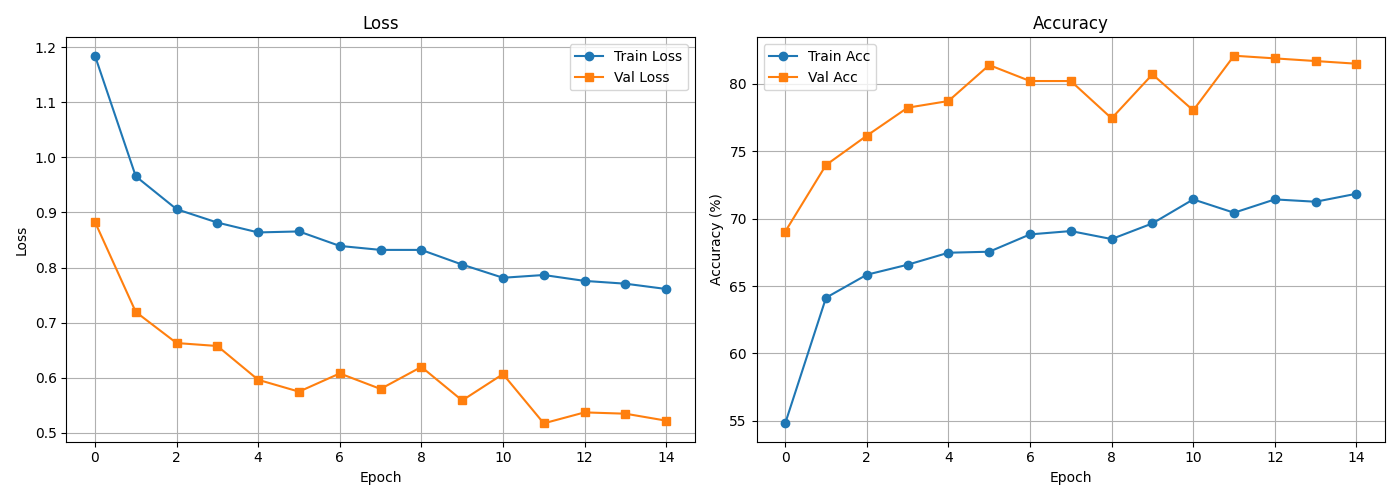
\includegraphics[width=\textwidth]{training_history.png}
\caption{Training and validation loss (left) and accuracy (right) over 15 epochs.}
\label{fig:training}
\end{figure}

Figure~\ref{fig:confusion} shows the confusion matrix on the test set. Cardboard (139/153, 91\%) and paper (208/244, 85\%) achieved the highest per-class accuracy. Glass was frequently confused with metal (27 misclassifications), and plastic was often misclassified as glass (34 cases). The ``trash'' category performed worst (18/45, 40\%), likely due to its small sample size and visual inconsistency.

\begin{figure}[H]
\centering
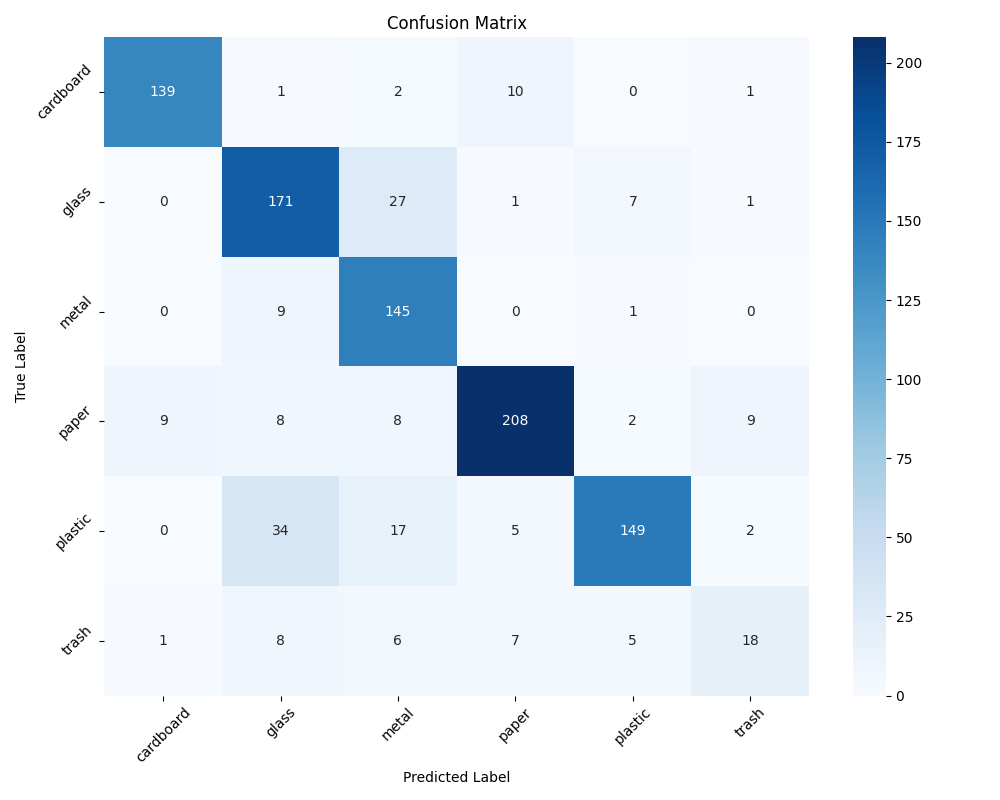
\includegraphics[width=0.75\textwidth]{confusion_matrix.png}
\caption{Confusion matrix on the TrashNet test set.}
\label{fig:confusion}
\end{figure}

\subsection{Real-World Swedish Waste Testing}

Testing on 17 Swedish waste items revealed a significant domain gap. Results are summarised in Table~\ref{tab:realworld}.

\begin{table}[H]
\centering
\caption{Real-world classification results on Swedish household waste tested in Gothenburg.}
\label{tab:realworld}
\begin{tabular}{lccc}
\toprule
\textbf{Category} & \textbf{Tested} & \textbf{Correct} & \textbf{Accuracy} \\
\midrule
Cardboard & 3 & 3 & 100\% \\
Paper     & 1 & 1 & 100\% \\
Plastic   & 4 & 1 & 25\% \\
Metal     & 7 & 6 & 86\% \\
Glass     & 2 & 0 & 0\% \\
\midrule
\textbf{Overall} & \textbf{17} & \textbf{11} & \textbf{65\%} \\
\bottomrule
\end{tabular}
\end{table}

Observations from real-world testing:

\begin{itemize}
  \item \textbf{Cardboard and paper} generalised well across domains (100\%). In the Swedish recycling system, cardboard and paper packaging (\textit{pappersf\"{o}rpackningar}) are collected together, so confusion between these two categories is not practically significant.
  \item \textbf{Plastic} performed poorly (25\%). Swedish plastic packaging differs from US packaging in colour, shape, and polymer type. Or might be caused by background color and lighting.
  \item \textbf{Glass} failed entirely (0\%). Transparency and reflections may also confuse the model.
  \item \textbf{Metal} was moderately successful (71\%). Clean metal surfaces were recognised well, but a metal can covered with a plastic wrapper was misclassified as cardboard.
  \item The \textbf{wooden background} may have influenced some predictions, as wood texture shares visual similarities with cardboard.
  \item \textbf{Zoom level} affected results: adjusting zoom sometimes improved classification accuracy.
\end{itemize}

\subsection{Hardware Demonstration}

The Arduino servo successfully responded to all classification outputs, rotating smoothly to the designated angle for each category. The system operated in real time with a 2-second capture interval, demonstrating the complete perception $\rightarrow$ cognition $\rightarrow$ action loop. A four-part demonstration video was produced covering software classification, hardware setup, and real-world testing. The demonstration used sample images from \citet{ozkefe2023waste} alongside the TrashNet dataset.

\section{Discussion}

The most significant finding is the \textbf{domain gap} between the US-sourced
TrashNet data and Swedish household waste. While the model achieved 82\% accuracy
on the benchmark, real-world accuracy dropped to 65\%. This is consistent with
known challenges in transfer learning: models that perform well on benchmark data
may underperform when deployed in a different cultural or geographic
context \citep{pan2010survey}. Although the small sample size of Swedish waste
items (17) limits statistical confidence of this test, the pattern is this: categories with
universal visual characteristics (cardboard, paper) transferred well, while
culturally variable categories (plastic, glass) did not. This suggests that fine-tuning on local data would benefit these weaker categories.
The confusion matrix from benchmark testing (Figure~\ref{fig:confusion}) already hinted at this weakness: plastic was frequently confused with glass (34 cases), and glass with metal (27 cases). These confusions were amplified in real-world testing where the visual characteristics of the items deviated further from the training distribution.

A further finding is that standardised image capture conditions are important.
In a production robot, a controlled environment with consistent lighting and
a neutral background could improve results. Additionally, a
multi-capture voting mechanism where multiple images are taken from
different angles and the system only acts when a majority agree on the same
material could increase classification confidence and reduce errors caused
by single misleading frames.

An interesting observation from the training curves (Figure~\ref{fig:training}) is that validation accuracy consistently exceeded training accuracy. This occurs because dropout is active during training (randomly disabling 50\% then 30\% of neurons) but disabled during evaluation. The frozen pre-trained layers also mean the model has strong generalisation from ImageNet features even while the trainable classification head is still adapting.

Hardware integration revealed challenges not visible in pure software testing. The Arduino resets when a serial connection is opened, requiring a 2-second initialisation delay. Power supply issues caused servo jitter when powered solely through USB, a breadboard and power supply module solved it easily. 

\subsection{Limitations}

\begin{itemize}
  \item Small and geographically biased training dataset (2,527 images, US-only).
  \item Uncontrolled capture environment (wooden background, variable indoor lighting, different zoom levels).
  \item Small real-world test set (17 items) limits statistical confidence.
  \item Screen capture pipeline rather than direct camera input adds latency and potential quality loss.
  \item Single servo motor demonstrates the concept but does not constitute a functional multi-bin sorting mechanism.
\end{itemize}

\section{Conclusion}

This project successfully demonstrates a proof-of-concept embodied AI system for waste sorting that implements the full perception $\rightarrow$ cognition $\rightarrow$ action loop. The ResNet18 transfer learning approach achieves 82.10\% accuracy on the TrashNet benchmark, but the domain gap between US training data and Swedish waste reduces real-world accuracy to 65\%. Cardboard and paper transfer well across domains; plastic and glass do not.

The system validates the technical feasibility of the approach while clearly identifying the requirements for production deployment: region-specific training data, controlled imaging conditions, and industrial hardware.

\subsection{Future Work}

\begin{itemize}
  \item Fine-tune the model on a Swedish or European waste dataset to close the domain gap.
  \item Use controlled lighting and a neutral background to reduce environmental interference.
  \item Replace the screen capture pipeline with a direct camera feed for lower latency.
  \item Upgrade to industrial servo motors and a multi-bin sorting mechanism.
  \item Expand the real-world test set for statistically solid evaluation.
  \item Explore attention mechanisms to help the model focus on material texture rather than packaging design.
\end{itemize}

\bibliographystyle{plainnat}
\bibliography{references}

\end{document}